\chapter{Sisteme încorporate}
\label{ch:embed}

După epoca calculatoarelor mainframe, urmată de o perioadă în care computerele
personale au condus lumea tehnologiei, ne îndreptăm spre perioada
calculatoarelor omniprezente (termenul a fost introdus pentru prima oară în 1988
de Mark D. Weiser, cercetător la Xerox PARC), când suntem înconjurați de
calculatoare de dimensiuni tot mai mici, comparabile chiar cu dimensiunile unei
monede.

Această evoluție se reflectă în popularitatea pe care a câștigat-o domeniul
Internet of Things (IoT) \abbrev{IoT}{Internet of Things} și evoluția
dispozitivelor inteligente. În prezent, dezvoltările tehnologiei se concentrează
pe realizarea unor dispozitive care să se adapteze cât mai mult necesităților
noastre și care să acționeze autonom, preluând cât mai multe din sarcinile
noastre. Suntem înconjurați de reclame la aspiratoare inteligente care își
construiesc o hartă a casei, parcurg întreaga suprafață și se conectează
singure la încărcător. Purtăm pe încheietura mâinii ceasuri și brățări care ne
monitorizează activitatea zilnică și ne avertizează când nu am făcut destulă
mișcare sau stăm pe scaun de prea mult timp.

Ca să ne facem o idee mai clară asupra popularității acestor dispozitive, un
studiu al World Economic Forum\footnote{\url{https://www.weforum.org/agenda/2019/04/why-securing-the-internet-of-things-is-crucial-to-the-fourth-industrial-revolution/}} indică folosirea a peste 14 miliarde de dispozitive în 2019, cu o estimare de 25 de miliarde în 2021.

În acest context, e ușor de observat o nevoie accelerată de a folosi sisteme de
calcul tot mai mici. Toate aceste sisteme inteligente pe care le integrăm
în viața noastră sunt, de fapt, niște roboți sau niște
calculatoare de dimensiuni reduse. Fiecare astfel de dispozitiv conține o
unitate de procesare și o memorie internă; mai specific, în componența
dispozitivelor inteligente intră sistemele încorporate.

Un sistem încorporat (\textit{embedded system}) este un sistem de calcul care controlează un proces. Spre
deosebire de calculatoarele clasice, aceste sisteme nu sunt dezvoltate pentru a
fi conectate la un monitor și o tastatură și controlate pentru operații diverse.
Sistemele încorporate sunt create cu un scop bine definit și sunt
adaptate pentru a deservi cât mai eficient acel scop, fie că sunt folosite
pentru a controla o bandă de asamblare sau o brățară care măsoară activitatea
fizică a unei persoane.

Sistemele încorporate stau la baza dispozitivelor inteligente și a platformelor
IoT, ele având dimensiuni, memorie, capacitate de procesare și conectivitate
adaptate sistemelor în componența cărora intră.

Un sistem IoT este un sistem de obiecte, dispozitive sau mașini interconectate
care este conectat și la Internet. Rețeaua permite acestor ,,lucruri'' să comunice
între ele și să furnizeze informații valoroase despre mediul înconjurător în
care sunt plasate.

\section{Microcontrolere și calculatoare}
\label{sec:embed:micro-comp}

Dispozitivele care controlează sisteme
inteligente sau anumite operații specializate sunt numite dispozitive
încorporate. Acestea sunt în principal unități de calcul având, de obicei,
caracteristici reduse, mai puțină putere de procesare și mai puțină memorie față
de calculatoarele cu care suntem obișnuiți. Multe dintre aceste sisteme sunt
similare cu calculatoarele pe care foloseam cu 15 sau 20 de ani în urmă, dar
care sunt proiectate să funcționeze în condiții speciale. Aceste dispozitive
integrate trebuie să funcționeze continuu timp de luni sau chiar ani, deoarece
ele sunt încorporate într-un sistem autonom. În plus, multe dispozitive trebuie
să reziste la condiții dure de funcționare, cum ar fi temperaturi extreme,
umiditate sau chiar ploaie. Cu cât dispozitivele încorporate sunt mai robuste, cu
atât sunt și mai costisitoare. Există o mulțime de dispozitive
încorporate având un preț de aproximativ 15-20 dolari. De cele mai multe ori,
acestea sunt folosite pentru prototipare și în educație. Pe de altă parte,
sisteme cu capacități similare, dar adaptate unor condiții dificile, pot atinge
prețuri de 100 sau chiar și de 1000 de ori mai mari.

Unele dintre cele mai comune dispozitive integrate, folosite în special în
educație, sunt Raspberry Pi sau Arduino. Aceste două placi sunt cunoscute
datorită prețului lor scăzut și a rezistenței la scurtcircuite.

Un aspect important de menționat în ceea ce privește dispozitivele încorporate
este că aceste sisteme, deși aparent asemănătoare cu calculatoarele personale,
folosesc arhitecturi diferite. În timp ce calculatoarele personale se bazează pe
procesoare Intel (x86, x64), aceste dispozitive încorporează diverse procesoare
cum ar fi Intel, ARM sau MIPS. Astfel, aplicațiile pentru dispozitivele
integrate sunt uneori mai greu de portat.

\subsection{Microcontrolere}
\label{sec:embed:micro-comp:micro}

Cele mai simple sisteme încorporate sunt microcontrolerele.

După cum sugerează și numele, un microcontroler este un sistem de control de
mici dimensiuni, folosit într-un număr mare de obiecte sau aparate. Dintr-o
perspectivă de ansamblu, un microcontroler seamănă cu un mic computer care vine
cu periferice, memorie proprie și cel puțin un procesor (CPU - Unitatea centrală
de procesare) capabil să execute un program (numit \textit{firmware}). De obicei, în
cadrul unui sistem de control, senzorii și servomotoarele sunt conectate direct
la microcontroler. Acest lucru se datorează faptului că microcontrolerele sunt
concepute special pentru a oferi suport pentru conexiuni diferite la dispozitive
periferice variate. În același timp, aceste plăcuțe sunt capabile să comunice cu
un dispozitiv mai complex, cum ar fi un computer. În plus, microcontrolerele
sunt optimizate și din alte puncte de vedere: dimensiune, consum de energie,
costuri etc. În principiu, ele sunt simple, accesibile și utilizate cu un scop
clar definit.

Deoarece microcontrolerele sunt dispozitive simple, concepute pentru un scop
anume, acestea rulează o singură aplicație. Software-ul rulat de
microcontrolere se numește \textit{firmware}; îl putem defini ca ,,software creat special
pentru hardware''. Firmware-ul este stocat, de regulă, în memoria flash (ROM),
care este non-volatilă (adică păstrează datele chiar dacă dispozitivul este
oprit și repornit) și conține informații relevante despre modul în care ar
trebui să funcționeze sistemul. Putem deci să deducem că odată programat, un
microcontroler poate fi integrat într-un sistem și el va rula acel firmware
chiar dacă sistemul este rebootat.

Datorită faptului că aceste dispozitive sunt capabile să ruleze doar o singură
bucată de software (firmware-ul), putem realiza aplicații în timp real (aplicații
care necesită un răspuns instant la un declanșator extern). Practic, aceste
dispozitive nu au un sistem de operare, deci orice întreruperi provenite de la
un periferic sunt declanșate și procesate într-un timp exact stabilit. Aceasta
înseamnă că procesorul nu mai execută sarcinile curente și începe executarea
rutinelor legate de întrerupere. Dacă nu sunteți familiarizat cu conceptul de
întreruperi, vă puteți gândi la ele ca la semnalele provenite de la
dispozitivele periferice. Astfel, odată ce un dispozitiv periferic trimite un semnal,
acesta este tratat instantaneu. În plus, un alt avantaj de a avea doar o singură
bucată de software care rulează pe dispozitiv este faptul că putem prezice când
se execută o anumită instrucțiune.

\subsubsection{Conectori}
\label{sec:embed:micro-comp:micro:connect}

Principalul scop al microcontrolerelor este de a le conecta la senzori și
actuatori. Acest lucru se face de obicei prin intermediul unor conectori
speciali; în cazul dispozitivelor educaționale, conectorii sunt niște pini. Din
firmware, programatorii pot citi sau controla starea acestor pini. Un avantaj al
microcontrolerelor este faptul că expun pini foarte specializați. În
general, un microcontroler are în primul rând un set de pini meniți să
îndeplinească sarcini de bază: ei permit conexiuni la periferice simple și, în
fond, alimentează cu energie perifericele. Chiar dacă acest ,,pachet'' de pini de
bază este găsit pe aproape fiecare microcontroler, numărul și amplasarea lor
diferă de la dispozitiv la dispozitiv. Un singur pin este capabil să efectueze
mai multe funcții în același timp (acest fenomen este numit ,,multiplexare'').

Cei mai simpli pini pe care îi putem găsi pe dispozitivele încorporate sunt:

\begin{itemize}
  \item \texttt{Vcc} - Acești pini sunt practic o sursă de tensiune cu o valoare
    fixă. Ne putem gândi la ei ca la polul pozitiv al unei baterii.
    Nu pot fi controlați din firmware.
  \item \texttt{GND} - Acești pini sunt cei opuși celor \textit{Vcc}. Ei sunt masa
                dispozitivului, de aceea se numesc pini \textit{ground}; ei sunt
    referința față de care se calculează orice cădere de tensiune.
    Nu pot fi controlați din firmware.
  \item \texttt{GPIO} \abbrev{GPIO}{General Purpose Input Output} (\textit{General Purpose
                Input Output}) - Sunt pini simpli care pot fi controlați din
    firmware. În funcție de starea lor, ei pot să funcționeze fie ca
                pini \texttt{Vcc} sau \texttt{GND}, fie ca un voltmetru, citind date de la senzori.
  \item \texttt{ADC} \abbrev{ADC}{Analog to Digital Converter} (Analog to Digital
    Converter) - Sunt pini care preiau date de la senzori și le
    transformă în valori digitale. Valorile pot fi citite din
    firmware.
  \item \texttt{DAC} \abbrev{DAC}{Digital to Analog Converter} (Digital to Analog
                Converter) - Sunt pini asemănători cu cei de \texttt{Vcc}, dar care pot
                fi controlați din firmware să expună un voltaj între \texttt{0} și \texttt{Vcc};
    sunt folosiți pentru a controla periferice, cum ar fi motoare.
  \item \texttt{PWM} \abbrev{PWC}{Pulse Width Modulation} (\textit{Pulse Width Modulation})
    - Sunt pini care simulează comportamentul pinilor DAC, fiind mai
    ieftini. Aceștia oscilează între GND și Vcc, simulând o tensiune
    variabilă.
\end{itemize}

Pe de altă parte, există pini care controlează periferice mai complexe, ce
transmit și primesc date folosind diverse protocoale:

\begin{itemize}
  \item \texttt{SDA} + \texttt{SCL} - câte doi pini pentru fiecare canal de comunicație I$^2$C; detalii despre I$^2$C în \labelindexref{Secțiunea}{sec:embed:bus:wired:i2c}
  \item \texttt{SCK} + \texttt{MOSI} + \texttt{MISO} - câte trei pini pentru fiecare canal de
          comunicație SPI suportat; detalii despre SPI în \labelindexref{Secțiunea}{sec:embed:bus:wired:spi}
  \item \texttt{TX} + \texttt{RX} - câte doi pini pentru fiecare canal serial suportat.
\end{itemize}

\subsubsection{Exemple de microcontrolere}
\label{sec:embed:micro-comp:micro:example}

Cum am menționat deja, există o varietate foarte mare de microcontrolere pe
piață, de la cele dezvoltate pentru a fi integrate în sisteme industriale, la
plăcuțe simple care se folosesc pentru prototipare sau în educație:

\begin{itemize}
  \item Arduino - Este o placă cu un microcontroler ATMega produs de o
    companie italiană. Este cel mai popular sistem de microcontroler
    utilizat pentru prototipuri și în scopuri educaționale. De fapt,
    Arduino constă atât în plăcuța efectivă, cât și în mediul
    integrat de dezvoltare (IDE), care ușurează procesul de
    programare al dispozitivului. Arduino și-a câștigat
    popularitatea chiar datorită IDE-ul foarte ușor de folosit, nu
    neapărat datorită produsului hardware.
  \item ESP32 - Este un microcontroler foarte ieftin cu WiFi integrat care este folosit
    în general ca \textit{placa de rețea pentru microcontrolere}. Acestă placă se conectează la
    alte microcontrolere prin portul serial și permite acestora accesul la Internet.
  \item MicroBit - Este o placă dezvoltata de BBC în scopuri educaționale ce are 
    un microcontroler nRF52 produs de Nordic Semiconductor. Este mai adecvat pentru
    a începe programarea pe microcontrolere, dar poate fi folosit și pentru
    proiecte mai mari.
\end{itemize}

\subsection{Calculatoare integrate}
\label{sec:embed:micro-comp:embed}

Am descris deja microcontrolerele ca fiind dispozitive simple utilizate cu un
scop clar definit. Tocmai datorită capabilităților reduse ale microcontrolerelor,
acestea nu au de obicei acces la rețea. În plus, chiar dacă am avea acces la un
microcontroler care suportă o conexiune la rețea, integrarea acestuia într-un
sistem IoT ar reprezenta un risc de securitate. Din cauza memoriei reduse,
microcontrolerele nu sunt capabile să implementeze protocoale securizate sau
alte mecanisme de securitate. Prin urmare, folosind un microcontroler am obține
un sistem care transferă date nesecurizate. Ținând cont de acest lucru, este
clar că nu putem proiecta o soluție IoT bazată exclusiv pe microcontrolere.

Un calculator încorporat reprezintă un sistem de calcul de dimensiuni mici, de
obicei foarte personalizat pentru a deservi unor scopuri specifice. Acest tip de
dispozitive este utilizat în mod obișnuit ca parte a unui alt sistem (cum ar fi
un ceas inteligent, un bancomat sau chiar un autoturism) care îndeplinește
sarcini complexe. Deși aceste dispozitive sunt de fapt calculatoare, în
majoritatea cazurilor, acestea nu suportă o interfață de utilizator, consumă
cantități mici de energie și dispun de resurse limitate de calcul.

Fiind calculatoare, spre deosebire de microcontrolere, dispozitivele rulează un
sistem de operare care gestionează resursele.

Unul din scopurile principale ale calculatoarelor integrate este de a trimite
sau de a prelua date din rețeaua locală sau chiar de pe Internet. De aceea,
aceste dispozitive au, în general, integrată o placă de rețea. Datorită memoriei
și puterii de procesare crescute față de un microcontroler, calculatoarele
integrate implementează mecanisme de securitate pentru transferul
de date și pentru aplicațiile rulate. Acest lucru permite dispozitivelor să
devină ,,inteligente'' și să comunice între ele.

În plus, calculatoarele încorporate sunt capabile să execute aplicații în
paralel. Pe de altă parte, datorită sistemului de operare care gestionează
resursele hardware și software, aceste dispozitive încorporate nu pot rula
aplicații în timp real. Acesta este un dezavantaj față de microcontrolere.

Pentru anumite proiecte simple, putem folosi calculatoare integrate în locul
microcontrolerelor. Acest lucru se datorează faptului că și aceste dispozitive
expun anumiți pini. Scopul pinilor este de a controla câteva periferice simple,
pentru interacțiunea cu utilizatorul (de exemplu, unele LED-uri
\abbrev{LED}{Light-Emitting Diode} care semnalizează starea sistemului). De
obicei, numărul de pini expuși de calculatoarele integrate este limitat,
majoritatea fiind pini GPIO. Aceste dispozitive nu expun mulți pini
pentru că scopul lor principal nu este acela de a interacționa cu mediul, ci de
a aduna, procesa și transporta date. Adăugarea unor module de conectare, cum ar
fi ADC sau DAC, crește prețul dispozitivului fără a-i crește în mod semnificativ
valoarea. Pe de altă parte, aproape toate sistemele de calcul încorporate
dispun de conexiuni avansate cum ar fi SPI, I$^2$C, USB, UART sau chiar HDMI. Pentru
a fi ușor de controlat, unele calculatoare integrate pot fi conectate la un
monitor, o tastatură și un mouse, similar unui calculator obișnuit.

\subsubsection{Exemple de calculatoare integrate}
\label{sec:embed:micro-comp:embed:example}

Avem o diversitate mare de calculatoare integrate pe care le putem folosi în
cadrul sistemelor inteligente:

\begin{itemize}
  \item Raspberry Pi - Deși nu a fost primul calculator integrat,
    Raspberry Pi este cel mai cunoscut și a fost dispozitivul care a
    revoluționat domeniul IoT. Este primul calculator integrat
    dedicat publicului larg, având un preț scăzut, ceea ce a dus la
    o scădere generală a prețurilor la alte dispozitive similare și
    a făcut domeniul IoT accesibil pasionaților de tehnologie și în
    educație. Dispozitivul costă aproximativ 35 de dolari.
  \item BeagleBone Black - BeagleBone Black este un dispozitiv cu
    capabilități de procesare mai scăzute în comparație cu Raspberry
    Pi. Cu toate acestea, dispozitivul expune un număr mai mare și
    mai variat de pini. BeagleBone Black poate fi folosit cu
    ușurință pentru prototipuri, dar poate fi integrat și în aparate
    inteligente, cum ar fi cabine foto sau frigidere inteligente.
    Dispozitivul costă în jur de 45 de dolari.
  \item Raspberry Pi Compute Module - Este un Raspberry Pi pentru uz
    industrial.
\end{itemize}

\subsubsection{Sisteme de operare pentru calculatoarele integrate}
\label{sec:embed:micro-comp:embed:os}

După cum am precizat anterior, calculatoarele integrate sunt mai mici și mai
ieftine, dar cu o putere de calcul și o memorie mai mică comparativ cu un
calculator de dimensiuni mari. Raspberry Pi, de exemplu, are 1GB de memorie RAM
în timp ce BeagleBone Black are 512 MB. Microprocesoarele acestor dispozitive au
frecvențe la o treime din frecvența unui calculator personal. Acest lucru le
permite să utilizeze o cantitate mică de energie și să fie accesibile ca preț.
Pe de altă parte, acest aspect duce la nevoia de a avea sisteme de operare
specializate, care să gestioneze cât mai eficient resursele disponibile. Aceste
dispozitive au nevoie de un sistem de operare foarte eficient în ceea ce
privește consumul de energie, deoarece funcționează de obicei pe baterie
și trebuie să fie autonome pentru perioade lungi de timp.

\textbf{Linux}

Știm deja că Linux e o platformă foarte utilizată și pentru calculatoarele
personale. În timp, odată cu evoluția IoT, s-au dezvoltat foarte multe
distribuții Linux pentru calculatoare integrate:

\begin{itemize}
  \item Raspbian - Este sistemul de operare recomandat pentru Raspberry
    Pi. A fost dezvoltat de Fundația Raspberry Pi. Ca orice alt
    sistem de operare, Raspbian suportă controlul dispozitivului
    prin Shell, folosind comenzile standard Linux. Raspbian vine în
    două versiuni: Desktop și Lite.
  \item Desktop este bazat pe Debian Linux și este optimizat pentru
    Raspberry Pi. Distribuția oferă inclusiv o interfață grafică de
    utilizator (GUI) și câteva aplicații, cum ar fi Chromium,
    LibreOffice și Claws Mail. Există și o versiunea Desktop care include
    preinstalate mai multe aplicații.
  \item Lite este versiunea Stretch fără GUI, având dimensiuni
    reduse. Interacțiunea cu sistemul se realizează doar prin linie
    de comandă.
  \item Ubuntu Server - Este sistemul Ubuntu Server compilat pentru Raspberry Pi, 
    practic identic cu sistemul destinat calculatoarelor server sau desktop.
  \item Ubuntu Core - Este un sistem de operare bazat pe Ubuntu. Spre deosebire
    de Ubuntu Server, Core este special realizat pentru sisteme IoT.
    Acesta include doar sistemul de pachete \textit{snap} si oferă posibilitatea
    aducerii la zi a sistemului de la distanță. Este în general utilizat 
    în scopuri industriale.
  \item Yocto - Yocto este un set de instrumente open source pentru
    crearea de imagini de sisteme de operare bazate pe Linux pentru
    dispozitivele încorporate. Sistemul include medii de emulare și
    depanatoare. Yocto a devenit popular pe piața hobbyștilor când
    Intel a lansat dispozitivele Edison și Galileo, ambele având o
    distribuție Yocto. Este un sistem compatibil cu Raspberry Pi.
\end{itemize}

\textbf{Sisteme de operare în timp real (Real-time Operating Systems - RTOS)}

Această categorie constă în sisteme de operare construite de la zero, special
pentru dispozitive încorporate. După cum sugerează și numele acestora, aceste
sisteme de operare vizează susținerea aplicațiilor în timp real. Ele
implementează algoritmi de programare speciali care se asigură că orice
eveniment extern este tratat imediat. Sistemele de operare în timp real existente
nu au nimic în comun, cu excepția faptului că toate sunt proiectate în același
scop. În contrast cu cele două categorii anterioare, exemplele pe care le vom
menționa nu împărtășesc același nucleu:

\begin{itemize}
  \item FreeRTOS este un sistem de operare open source mențiunt de către Amazon. 
    Este cel mai vechi sistem de acest gen, considerat ca fiind cel mai potrivit
    pentru uz industrial. Este scris in C și este axat pe performanță.
  \item Zephyr Project este un sistem de operare open source insiprat din Linux și realizat
    inițial de către Intel. Este considerat \textit{fratele mai mic al Linuxului}.
    Deși este inspirat din Linux, funcționarea acestuia este foarte diferită, acesta fiind
    conceput ca un sistem de operare în timp real. Fiind mai nou decât FreeRTOS și având 
    un API similar cu Linux, acesta este recomandarea actuală pentru folosirea în industrie.
  \item RIOT este un sistem de operare open source. Arhitectura acestuia îl face ușor de
    adaptat la sistemele cu memorie redusă. RIOT este compatibil cu
    Raspberry Pi, Beagle Board, unele tipuri de Arduino (modele mai
    avansate care sunt mai mult decât un microcontroler și au o
    putere de calcul mai mare).
  \item Contiki - Contiki este un sistem de operare open source dezvoltat
    special pentru sisteme IoT de Texas Instruments. Principalul său
    avantaj față de alte sisteme de operare similare este consumul
    redus de energie și de memorie.
  \item Tock este primul sistem de operare folosit în industrie scris într-un alt
    limbaj decât C, mai exact Rust. De asemenea, este primul sistem de operare
    pentru micrcontrolere care face o separare clară între kernel și aplicații.
    Tock este folosit de către Google în proiectul OpenSK și de către 
    proiectul OpenTitan.
\end{itemize}

\section{Sisteme simple de intrare ieșire}
\label{sec:embed:io}

Având în vedere faptul că sistemele inteligente au drept scop extragerea de
informații despre mediul înconjurător și interacțiunea cu acesta, este necesară
integrarea senzorilor și a actuatorilor în aceste sisteme.

Un senzor este o componentă electronică sau un modul destinat să urmărească
evenimente sau modificări din mediu și să transmită datele colectate unui alt
dispozitiv. Exemple sunt senzori de temperatura, de umiditate, butoane, senzori
de lumina etc.

Un actuator este un element de acționare care aduce modificări asupra mediului.
Un exemplu foarte bun este un LED.

Aceste sisteme de intrare/ieșire sunt perifericele specifice dispozitivelor
încorporate, deci una din caracteristicile principale ale unui dispozitiv
încorporat este capacitatea de realiza conexiuni la aceste periferice.

În dezvoltarea sistemelor inteligente putem alege între mai multe tipuri de
periferice în funcție de modul în care acestea se conectează și schimbă date cu
dispozitivul încorporat. Există periferice simple care comunică direct cu
dispozitivul la care sunt conectate sau există unele mai complexe care au o
unitate de procesare integrată (un microcontroler), permițând un schimb mai
complex de mesaje.

Din punct de vedere al datelor furnizate dispozitivului la care sunt conectate,
perifericele pot să fie digitale sau analogice (se trimit semnale digitale sau
analogice).

Semnalele care sunt continue în timp sunt considerate semnale analogice, în timp
ce semnalele care iau valori discrete sunt considerate semnale digitale.
Considerăm că un semnal este continuu dacă acesta poate să ia orice valoare
într-un anumit interval.

Dacă, de exemplu, semnalul nostru poate lua orice valoare în intervalul [2; 5]
(2; 2.1; 2.11; 2.11111; 3.(4); și așa mai departe) este un semnal analogic. Dacă
avem un semnal discret, el poate lua doar anumite valori. De exemplu, dacă
semnalul nostru poate lua doar valorile {1; 0} (pornit / oprit) sau poate lua
doar valorile {2; 3; 4; 5; 100}, el este digital.

\begin{figure}[htbp]
  \centering
  \def\svgwidth{\columnwidth}
  \includesvg{chapters/15-embed/img/analog-digiat.svg}
  \caption{Semnal analogic vs. semnal digital}
  \label{fig:embed-analog-digital}
\end{figure}

Cum am precizat mai sus, dispozitivele încorporate, cum ar fi Raspberry Pi sau
Arduino, expun pini la care aceste sisteme de intrare/ieșire se pot conecta. În
funcție de semnalul pe care perifericul îl transmite, el trebuie conectat la
anumiți pini (nu putem conecta un senzor care transmite un semnal analogic la un
pin care suportă doar semnale digitale).

Cei mai simpli pini sunt cei care sunt folosiți pentru semnale digitale. Ei se numesc pini
GPIO (\textit{General Purpuse Input/Output}) și pot să funcționeze în două moduri, ca
intrare sau ca ieșire.

În cazul în care un pin GPIO funcționează ca o ieșire digitală, el poate fi
conectat la un sistem de acționare pe care îl controlăm prin intermediul
pinului. În acest caz, pinul funcționează ca o baterie și poate să înlocuiască
fie borna pozitivă, fie borna negativă a bateriei. În general, vom seta pinul în
starea \textit{HIGH} (1), în care va funcționa ca o bornă pozitivă, sau \textit{LOW} (0), în care
va funcționa ca o borna negativă (sau ca un pin de ground).

Cel mai simplu exemplu de folosire pentru acești pini este controlul unui LED.
Un LED este o componentă electronică (o diodă) care generează lumină când este
străbătută de curent. Deci, pentru a face un LED să lumineze, e suficient să îl
conectăm la o baterie.

\begin{figure}[!htbp]
  \centering
  \includegraphics[width=0.6\textwidth]{chapters/15-embed/img/raspberry-img.png}
  \caption{LED conectat la Raspberry Pi}
  \label{fig:embed:raspberry}
\end{figure}

\labelindexref{Figura}{fig:embed:raspberry} conține un LED conectat la pinii
unui Raspberry Pi. Unul din pini este conectat la ground (borna negativă a
bateriei), iar celălalt este conectat la un pin GPIO. Dacă scriem valoarea 1 pe
pin, acesta va genera un voltaj și LED-ul va începe să lumineze. Dacă scriem
valoarea 0 pe pin, acesta va fi practic conectat la două borne negative, deci nu
va lumina. Jonglând cu aceste două stări putem face diverse jocuri de lumini.

Pe de altă parte, putem folosi un pin digital ca intrare. În acest caz, el se
comportă ca un voltmetru care măsoară diferența de potențial relativ la
groundul plăcii, adică tensiunea la nivelul pinului. Dacă tensiunea este mai
mică decât jumătate din valoarea maximă suportată de placă (\texttt{Vcc/2}), pinul va
raporta valoarea 0. În caz contrar, se va raporta valoarea 1.

Putem, de exemplu, să conectăm un buton la un astfel de pin și să citim starea
butonului. În general, dacă butonul va fi apăsat vom citi o tensiune apropiată
de tensiunea maximă a plăcii, iar dacă butonul nu este apăsat, tensiunea va fi
aproape 0.

Pinii GPIO sunt utili în interacțiunea cu periferice simple cum ar fi LED-uri
sau butoane, dar majoritatea senzorilor și a elementelor de acționare nu
funcționează atât de ușor. Pentru perifericele mai complexe avem la dispoziție
pini analogici și PWM.

În general, senzorii sunt rezistențe variabile care își modifică valoarea în
funcție de factorii de mediu. Astfel, căderea de tensiune de pe senzor se
schimbă.

Pinii analogici funcționează ca un voltmetru care măsoară căderea de tensiune de
pe senzor și o transformă într-o valoare finită. Dispozitivul care face
conversia din voltaj într-o valoare întreagă, transmisă plăcii, se numește
\textbf{convertor analog-digital} (ADC). Valorile întregi returnate depind de numărul de
biți integrați în ADC. Dacă considerăm n numărul de biți al ADC-ului, valorile
sunt în intervalul \texttt{0-$2^{n-1}$}. De exemplu, convertorul analog-digital integrat
în plăcuțele Arduino are 10 biți, deci valorile citite de pe pinii analogici
sunt în intervalul \texttt{0-1023}.

Putem astfel să conectăm un fotorezistor la un pin analog, iar în funcție de
luminozitatea mediului vom citi valori mai mici sau mai mari. Dacă identificăm o
luminozitate prea mică, putem scrie valoarea 1 pe un pin GPIO conectat la un LED
și să aprindem LED-ul, obținând un prototip al unui sistem de iluminare
inteligent.

Am stabilit că pentru a citi semnale analogice vom folosi pini conectați la un
ADC, dar ce facem pentru a trimite semnale analogice mediului?

În primul rând, există posibilitatea de a folosi un convertor digital-analogic
(DAC). El transformă o valoarea digitală într-un semnal analogic. Putem deci să
scriem o valoare pe un astfel de pin pentru a controla tensiunea de ieșire a
pinului. Astfel de pini sunt folosiți pentru a controla motoare.

Pe de altă parte, convertoarele de la digital la analogic sunt destul de scumpe,
de aceea multe dispozitive încorporate nu expun astfel de pini. În schimb, ele
folosesc o metodă mai accesibilă de simulare a semnalelor analogice, PWM.

\textit{Pulse Width Modulation} (PWM) este o modalitate de a simula semnale analogice
prin mijloace digitale. Putem realiza acest lucru prin alternarea rapidă între
semnale care pot avea doar două valori (0/1), dar prin modificarea factorului de
umplere, adică timpul în care pinul are valoarea 1. De multe ori, receptorul
semnalului va face o medie a celor două valori alternative.

De exemplu, dacă avem un LED care clipește foarte repede, ochiul uman îl va
percepe ca un LED ce luminează la o anumită intensitate. În funcție de raportul
între perioada în care LED-ul este aprins versus perioada de timp în care el
este stins, lumina va fi percepută la o intensitate mai mare sau mai joasă.

\begin{figure}[htbp]
  \centering
  \def\svgwidth{\columnwidth}
  \includesvg[width=0.7\textwidth]{chapters/15-embed/img/pwm.svg}
  \caption{Pulse Width Modulation (PWM)}
  \label{fig:embed-pwm}
\end{figure}

Acești pini pot fi folosiți pentru a controla LED-uri sau chiar motoare.

\section{Magistrale de comunicare}
\label{sec:embed:bus}

Până acum am enumerat modalitățile de conectare a perifericelor simple, folosind
pini digitali sau analogici. Cum am menționat deja, multe din perifericele
existente sunt sisteme complexe, care au un procesor integrat și care trimit
date structurate. În plus, există multe periferice care comunică wireless cu
dispozitivele încorporate.

Pentru a interacționa cu aceste dispozitive de intrare/ieșire complexe, există
diverse protocoale prin fir (ex. serial, SPI (\textit{Serial Pripheral Interface})\abbrev{SPI}{Serial Peripheral
Interface}, I$^2$C, Modbus, CAN (\textit{Controller Area Network})\abbrev{CAN}{Controller Area Network}) sau wireless
(ex. Bluetooth, Wi-Fi, LoRa, Z-Wave). Unele din aceste protocoale sunt valabile
și pentru calculatoarele clasice. De exemplu, porturile USB implementează o
conexiune serială. De asemenea, utilizăm zilnic mouse-uri wireless, unele
folosind Bluetooth pentru comunicare. Pe de altă parte, multe din protocoalele pe care
le vom descrie mai departe au fost implementate special pentru comunicarea între
dispozitivele încorporate și periferice.

\subsection{Comunicare prin fir}
\label{sec:embed:bus:wired}

Unele din primele periferice complexe au fost dezvoltate pentru a fi conectate
direct la calculatoare, transmisia făcându-se prin intermediul firelor. Cea mai
cunoscută astfel de conexiune este conexiunea serială.

În continuare vom descrie câteva din protocoalele pe care mulți senzori și alte
periferice le implementează.

\subsubsection{Comunicarea serială}
\label{sec:embed:bus:wired:serial}

Comunicarea serială (\labelindexref{Figura}{fig:embed:serial}) e unul dintre cele mai cunoscute și simple protocoale.
Protocolul presupune trimiterea datelor între dispozitive bit cu bit, pe rând.
În contrast, există linii de comunicație paralele, unde datele sunt trimise în
paralel. Avantajul comunicării seriale este simplitatea.

Pentru a implementa un protocol serial sunt necesare minim două linii de
comunicație, RX și TX. Pe fiecare linie se trimit date într-o direcție. Fiecare
dispozitiv trimite date pe TX și primește date pe linia RX. Astfel, când
conectăm două dispozitive, linia RX a unuia se va conecta la linia TX a
celuilalt și invers.

\begin{figure}[htbp]
  \centering
  \def\svgwidth{\columnwidth}
  \includesvg[width=0.7\textwidth]{chapters/15-embed/img/serial.svg}
  \caption{Conexiune serială}
  \label{fig:embed:serial}
\end{figure}

Pentru a se asigura un transfer corect de date, protocolul serial se bazează pe
următoarele elemente:

\begin{itemize}
  \item biți de date - datele efective transmise între dispozitive;
  \item biți de sincronizare - sunt biți transmiși înaintea și după biții
    de date, pentru a marca începutul și sfârșitul blocului de date;
  \item biți de paritate - e o modalitate simplă de a face verificarea
    datelor transmise (o sumă de control foarte simplă); dacă trimitem 8
    biți de date și din acei 8 biți 5 conțin valoarea 1, datele
    trimise conțin un număr impar de valori de 1, deci bitul de
    paritate va fi setat la 1, dacă numărul de valori de 1 este par,
    bitul de paritate va fi setat la 0;
  \item baud rate - specifică viteza de transmitere a datelor; este foarte
    important ca ambele dispozitive conectate să transmită date la
    aceeași viteză.
\end{itemize}

Protocolul serial poate fi folosit doar la comunicarea între două dispozitive.
Asta înseamnă că fiecare dispozitiv periferic conectat are nevoie de un port
serial separat, făcând conectarea multor dispozitive nepractică.

\subsubsection{SPI}
\label{sec:embed:bus:wired:spi}

SPI e un protocol mai complex, care necesită 3 linii pentru comunicare. Datele
sunt transmise pe liniile MISO \abbrev{MISO}{Master In Slave Out}(\textit{Master In
Slave Out}) și MOSI \abbrev{MOSI}{Master Out Slave In} (\textit{Master Out Slave In}). Cea
de-a treia linie este folosită pentru sincronizare (\texttt{SCLK}).

SPI vine ca o îmbunătățire a conexiunii seriale, încercând să asigure
sincronizarea celor două dispozitive care comunică, transmisia de date
realizându-se într-un mod mai eficient prin reducerea erorilor rezultate de la
transmisie. Astfel, SPI se folosește de o a treia linie de comunicare dedicată
sincronizării transmisiei de date.

Un alt avantaj al SPI e că are suport pentru mai multe periferice, denumite \textit{slave},
conectate la un dispozitiv principal, numit \textit{master}. Fiecare dispozitiv este
activat sau dezactivat la un moment dat folosind un pin GPIO oarecare setat la
valoare 0 sau 1.

\subsubsection{I$^2$C}
\label{sec:embed:bus:wired:i2c}

I$^2$C, sau IIC (\textit{Inter-Integrated Circuit}) \abbrev{IIC}{Inter-Integrated Circuit}, e un
alt protocol care necesită două linii pentru transmiterea de date, SDA și SCL.
SDA e linia pe care se transmit efectiv datele, în timp ce SCL e linia de
sincronizare.

Avantajul protocolului I$^2$C este că putem conecta mai multe dispozitive simultan.
Avem dispozitive master și slave. În cazul I$^2$C este foarte importantă
sincronizarea dintre dispozitive. Avem o singură linie pe care se trimit toate
datele. De aceea, comunicarea este mereu inițiată de un master care cere
informații de la unul din dispozitivele slave conectate.

Fiecare dispozitiv are o adresă formată din 7 biți, adresă înregistrată în
periferic. Sistemul master interoghează pe rând fiecare adresă, putând astfel să
descopere adresele tuturor dispozitivelor legate la sistem.

\subsubsection{Alte protocoale folosite industrial}
\label{sec:embed:bus:wired:other}

\textbf{Modbus}

Un protocol folosit destul de mult in industrie este ModBus. Spre deosebire de
cele enumerate anterior, acesta este un protocol software. El definește cum
arată datele transmise între dispozitive, fără a defini însă o infrastructură
de comunicație. Există diferite variante, în funcție de ce mijloc de transport
de date se folosește. Exemple sunt o legătură serială sau Ethernet (rețea).
Similar cu I$^2$C, fiecare periferic conectat la Modbus are o adresă unică.

\textbf{CAN}

Un protocol folosit în industria Auto este CAN (\textit{Car Area Network}). Acesta leagă sistemele de control
din autoturisme de periferice. Aproape toate sistemele electronice din
autoturisme sunt legate la magistrala CAN. Fiecare
dispozitiv conectat la magistrală se numește nod. Fiecare nod are un ID (adresă)
unic. Protocolul are o variantă de viteză redusă, tolerantă la
erori. Protocolul a fost gândit pentru transmisie în timp real.

\subsection{Comunicarea wireless}
\label{sec:embed:bus:wireless}

Pe măsură ce platformele IoT au evoluat, ele au fost incluse în multe sisteme
întinse pe arii largi, cum ar fi sistemele agricole. Pentru astfel de cazuri,
conectarea fizică a senzorilor la sistemele de procesare este costisitoare și
consumă mult timp. Drept urmare, au fost implementate o mulțime de
microcontrolere și calculatoare integrate care suportă conexiuni WiFi. Cu toate
acestea, deoarece multe dintre dispozitivele utilizate în sistemele inteligente
funcționează pe baterie, a existat necesitatea unui protocol care să implice
consum redus de energie. Astfel, au apărut mai multe protocoale wireless,
special concepute pentru IoT.

\subsubsection{Bluetooth}
\label{sec:embed:bus:wireless:bluetooth}

Acesta a fost unul dintre primele protocoale implementate în sistemele IoT. Pe
măsură ce domeniul s-a dezvoltat și Bluetooth a rămas principalul protocol de
comunicare între dispozitive, acesta a fost extins, implementându-se Bluetooth
4.0, sau \textit{Bluetooth Low Energy} (BLE) \abbrev{BLE}{Bluetooth Low Energy}. Acesta
este special conceput pentru a consuma puțină energie în procesul de transfer al
datelor.

\subsubsection{Z-wave}
\label{sec:embed:bus:wireless:zwave}

Este un protocol utilizat în principal
pentru sistemele de automatizare a caselor (întrerupătoare, termostate,
încuietori inteligente). Comunicația între dispozitive se face prin unde radio,
iar dispozitivele trebuie să fie amplasate la o distanță de maxim 100 m.

\subsubsection{Sigfox}
\label{sec:embed:bus:wireless:sigfox}

Este un protocol conceput
pentru transmiterea de date între dispozitive situate la distanțe considerabile
unul de celălalt. Principalul avantaj al Sigfox este că poate fi utilizat în
agricultură sau în alte domenii în care dispozitivele trebuie să transmită date
pe distanțe mari. Folosind Sigfox, putem transmite date pe distanțe de până la
50 km în câmp deschis.

\subsubsection{LoRa}
\label{sec:embed:bus:wireless:lora}

Numele protocolului provine de la sintagma Long Range, rază lungă. Este similar cu
Sigfox, permițând schimbul de pachete pe distanțe lungi, până la 50 km în câmp
deschis, folosind foarte puțină energie pentru transmiterea de date.

\subsection{Sisteme Gateway}
\label{sec:embed:bus:gateway}

Pentru a permite acestor periferice să trimită și să primească date de la
dispozitivele integrate, cele două părți trebuie să implementeze același
protocol. Prin urmare, construirea unei soluții IoT care este, de exemplu,
compatibilă atât cu periferice LoRa, cât și cu periferice Sigfox, necesită implementarea celor
două protocoale în logica aplicației, iar introducerea unui al treilea protocol
necesită alt efort. De aceea, pentru comunicarea cu astfel de
periferice se folosesc, de obicei, gateway-uri. În general, gateway-urile sunt
dispozitivele care implementează protocolul de comunicație periferic, pe de o
parte, și un protocol TCP / IP standard, pe de altă parte, pentru a comunica cu
dispozitivul încorporat. Rezultatul este că aplicația care rulează pe
dispozitivul încorporat comunică doar cu gateway-urile, folosind un singur
protocol, și este independentă de senzorii conectați la sistem.

\section{Dezvoltarea programelor pentru sisteme integrate}
\label{sec:embed:dev}

În procesul de dezvoltare al aplicațiilor pentru sisteme integrate trebuie să
ținem cont de faptul că aplicația dezvoltată va funcționa pe o perioadă
îndelungată și pe un sistem autonom. Astfel, trebuie să ne asigurăm că orice
posibile erori sunt tratate cu atenție, fără a necesita intervenție umană.

Putem identifica următorii pași în dezvoltarea programelor pentru aceste
sisteme:

\begin{enumerate}
  \item scrierea programului
  \item testarea pe mai multe dispozitive
  \item instalarea aplicației pe toate dispozitivele necesare
  \item aducerea la zi a aplicației
\end{enumerate}

În ceea ce privește scrierea programului, procesul nu este diferit de cel pentru
aplicațiile obișnuite. În schimb procesul de rulare a aplicației pe dispozitiv
este diferit. Având în vedere că ne referim la dispozitive care nu au fost
concepute pentru interacțiunea directă cu utilizatorul, acestea nu au, în general,
interfață grafică. Practic, noi vom scrie programul folosind un calculator
obișnuit, după care vom încărca executabilul pe dispozitivul integrat.

Cel mai important aspect când vine vorba de rularea unei aplicații pe un astfel
de dispozitiv este că, de cele mai multe ori, arhitectura pe care vom rula nu este
aceea pe care compilăm aplicația. De exemplu, dacă scriem un program pentru un
Raspberry Pi, care are un procesor ARM, va trebui să generăm un executabil
pentru acest procesor. Având în vedere că executabilul este generat pe
calculatorul personal, cu arhitectură de procesor x86, avem nevoie de utilitare care permit
compilarea programelor pentru alte arhitecturi.

Procesul de compilare a unui program pentru a rula pe o altă arhitectură se
numește \textbf{cross-compiling}.

Odată generat executabilul, acesta trebuie transferat pe sistemul integrat,
sistem la care nu avem o conexiune directă. Astfel, sunt necesare utilitare
precum \texttt{scp}, care implementează copierea prin SSH, pentru a transfera fișierul executabil pe dispozitive. În plus, avem
nevoie de acces la dispozitiv pentru a putea rula efectiv executabilul. Cea mai
accesibilă metodă de a face acest lucru este să deschidem o conexiune SSH la
dispozitiv.

Odată ce avem versiunea finală a executabilului, acesta trebuie transferat pe
toate dispozitivele pe care urmează să le dăm în producție. Acest procedeu este
mai complicat, de aceea există platforme speciale pentru asa ceva, cum ar fi
Resin.io sau Android Things. Pentru a le folosi, trebuie să înregistrăm toate
dispozitivele în cadrul platformei, după care se folosește un sistem de
distribuție pentru a instala aplicația pe fiecare dispozitiv. În plus, aceste
platforme oferă posibilitatea de a aduce îmbunătățiri aplicației și de a aduce
la zi toate dispozitivele.

În ceea ce privește aducerea la zi, trebuie să ținem cont de faptul că
dispozitivele pe care lucrăm sunt în producție, integrate în diverse obiecte sau
sisteme în funcțiune. De aceea, este foarte important ca procesul de aducere la
zi să decurgă fără întreruperi și, dacă intervine vreo problemă, să ne
asigurăm că aceasta nu rezultă în imposibilitatea de a mai folosi aparatul în
cauză.

\section{Internet of Things}
\label{sec:embed:iot}

În prezent, una din cele mai răspândite noțiuni din domeniul IT este cea de
Internetul Lucrurilor (\textit{Internet of Things} sau pe scurt IoT). Acest cuvânt cheie
se referă la ideea de inteligență ambientală, unde suntem înconjurați de obiecte
și aparate inteligente care se adaptează nevoilor noastre și acționează în
consecință. Exemple de astfel de obiecte și aparate inteligente sunt lumini inteligente care funcționează pe baza luminozității
exterioare, asistenți controlați vocal sau mașini autonome. Scopul IoT
este să trăim într-un mediu în care aceste dispozitive inteligente sunt
integrate în jurul nostru, devenind imperceptibile, dar îmbunătățindu-ne stilul
de viață.

Cel mai potrivit termen care să descrie această situație spre care tinde
Internetul Lucrurilor este cel de calcul omniprezent (\textit{ubiquitous computing}).
Este conceptul care a precedat IoT-ul și care a fost introdus în jurul anului
1988 de Mark D. Weiser, cercetător la Xerox PARC. Chiar dacă în perioada
respectivă existau niște limitările hardware considerabile, Weiser a reușit să
anticipeze progresul care va veni. De asemenea, a publicat mai multe lucrări
în care descrie concepte similare cu cele din IoT, precum și riscurile pe
care un asemenea progres le aduce. În cadrul lucrării intitulată ,,Computerul
pentru secolul XXI'', Weiser menționează ideea că un computer omniprezent nu se
referă la un lucru pe care îl poți purta cu ușurință, ci mai degrabă la un lucru
care este o parte a traiului zilnic la un asemenea nivel încât nu îi mai
observăm prezența. Integrarea perfectă a computerelor în activitățile noastre
zilnice rămâne și în prezent o provocare continuă, la care evoluția tehnologică
se luptă să facă față. Unele din previziunile lui Mark Weiser menționează lupta
de a obține o tehnologie calmă, o problemă cu care ne confruntăm acum prin
asaltul de informații sau prin încălcarea frecventă a intimității noastre prin
cunoscutele atacuri cibernetice. Deși suntem departe de a atinge calmul
tehnologic, evoluțiile tehnologice încă au dificultăți în a îndeplini această nevoie.

Unul dintre primele dispozitive de uz zilnic care a fost conectat la Internet a
fost automatul de Coca-Cola de la Universitatea Carnegie Mellon. Aparatul a fost
dezvoltat la începutul anilor 1980 de un grup de studenți. Scopul studenților a
fost de a dezvolta o modalitate prin care să se poată verifica dacă automatul
este gol fără a necesita deplasarea inutilă. În zilele noastre, acest aparat
este considerat unul din primele sisteme inteligente.

În anul 2000, Kevin Ashton, co-fondator al Centrului Auto-ID din cadrul
Massachusetts Institute of Technology, lucra la ceea ce avea să devină Internetul
Lucrurilor (IoT), termen pe care l-a brevetat în anul 2002, împreună cu David L.
Brock. În acea perioadă, echipa lui Kevin Ashton lucra la o modalitate de
standardizare a identificării prin radiofrecvență (RFID - \textit{Radio-frequency identification}) prin conectarea
informațiilor obținute la Internet. În prezent există la nivel global
laboratoare Auto-ID care lucrează împreună la dezvoltarea de sisteme RFID și
IoT.

Popularitatea în creștere a IoT poate fi explicată prin dorința oamenilor de a automatiza cât
mai multe din sarcinile zilnice. De altfel, răspunsul este potrivit nu doar
pentru evoluția IoT, ci pentru evoluția tehnologică în general. De secole am
căutat metode de automatizare a muncii noastre prin intermediul mașinilor, la
fel cum în momentul de față ideea de a avea aspiratoare autonome sau frigidere
care fac singure cumpărăturile on-line este una foarte atrăgătoare. Ca rezultat,
companiile IT au investit mult în cercetare și dezvoltare în acest domeniu, ceea
ce a dus la scăderea prețului senzorilor, microcontrolerelor, gateway-urilor
etc., făcând soluțiile inteligente accesibile publicului larg.

Un aspect important pe care să îl luăm în calcul când discutăm despre
dispozitive inteligente este acela că un obiect inteligent nu e neapărat un
sistem IoT. Să luăm exemplul unor becuri inteligente, care luminează mai
puternic sau mai slab în funcție de lumina ambientală. Deși este evident că avem
un dispozitiv inteligent, care își adaptează comportamentul în funcție de
ambient și de nevoile noastre, sistemul nu este unul IoT, nu avem conectivitate
la Internet și nu conectăm mai multe sisteme diferite.

Fiind vorba despre dispozitive care comunică, pentru Internet of Things se poate
defini o stivă pentru a reprezenta traseul pe care datele sunt transmise. Deși
nu este definită ca un standard, se consideră, în general, că majoritatea
sistemelor Internet of Things au următoarea structură:

\begin{itemize}
  \item senzori și actuatori
  \item procesare și stocare locală
  \item conexiunea la Internet
  \item cloud
\end{itemize}

Acum, că suntem familiarizați cu caracteristicile unui sistem IoT, să aruncăm o
privire la unele dintre cele mai utilizate dispozitive inteligente din zilele
noastre. Este important să observăm modul în care urmăresc stiva IoT și care
este scopul final al acestora.

\subsection{Implementări de sisteme IoT}
\label{sec:embed:iot:impl}

\subsubsection{Amazon Alexa}
\label{sec:embed:iot:impl:alexa}

\begin{figure}[!htbp]
  \centering
  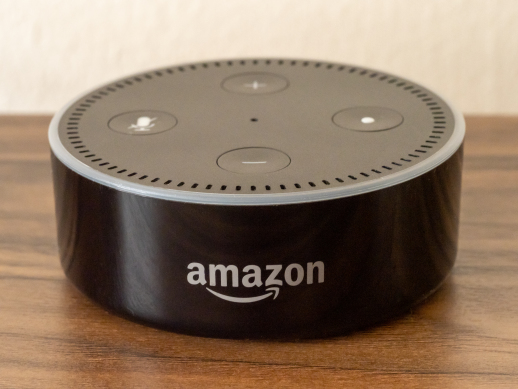
\includegraphics[width=0.8\textwidth]{chapters/15-embed/img/alexa.jpg}
  \caption{Amazon Alexa}
  \label{fig:embed:alexa}
\end{figure}

La o primă privire, soluția Alexa (în \labelindexref{Figura}{fig:embed:alexa}), dezvoltată de Amazon, nu pare nimic mai mult
decât un difuzor wireless. De fapt, sistemul este capabil să facă mult mai mult
decât redarea unor melodii, fiind un sistem complex de control vocal. Prin
intermediul Alexa, utilizatorii pot seta alarme, căuta articole pe
Wikipedia, pot obține informații în timp real despre condițiile
meteorologice și de trafic. În plus, Alexa poate funcționa și ca un sistem de
control al casei, fiind compatibil cu o gamă largă de dispozitive (becuri,
televizoare etc.).

Din punct de vedere tehnic, Alexa este un dispozitiv inteligent care utilizează
un microfon pentru a obține informații de la utilizator, trimite datele în
cloud, unde acestea sunt procesate - un asistent virtual (\textit{virtual assistant}). Odată ce sistemul din cloud ,,înțelege''
comanda, acesta generează răspunsul, fie că este vorba despre anumite informații
pe care le primește de pe Internet, fie despre unele acțiuni pe care
dispozitivul trebuie să le efectueze, și trimite răspunsul înapoi pe dispozitiv.

\subsubsection{Ceasuri inteligente}
\label{sec:embed:iot:impl:smartwatch}

Câteva din caracteristicile principale ale ceasurilor inteligente sunt comenzile
vocale, ghidarea pe hartă, redarea muzicii sau afișarea de mesaje text. Aceste
dispozitive pot realiza sarcini complexe, majoritatea fiind
dotate cu sisteme de operare mobile precum Android. Dimensiunile reduse și
utilitatea le transformă în ,,calculatoare portabile'' și chiar ,,telefoane care
pot fi purtate'', ultimele versiuni fiind capabile să răspundă și să efectueze
apeluri vocale și video.

În realitate, aceste sisteme sunt în general alcătuite din două componente:
ceasul inteligent și telefonul la care acesta se conectează. Ceasurile sunt de
fapt senzorii și ecranul care redă imagini, în timp ce telefoanele inteligente
sunt adevăratele dispozitive de procesare. Cele două comunică de obicei prin
Bluetooth 4.0. Provocarea principală în proiectarea acestui tip de dispozitive
este de a asigura consumul de energie cât mai redus posibil.

\subsubsection{Electrocasnice inteligente}
\label{sec:embed:iot:impl:home}

În ultima perioadă, electrocasnicele au devenit ,,inteligente'', ceea ce înseamnă
că se pot conecta la Internet într-un fel sau altul și, bineînțeles, pot
comunica între ele pentru a optimiza cantitatea de energie utilizată. Este vorba
de frigidere, mașini de spălat vase, aspiratoare sau termostate
inteligente. În general, funcționarea lor poate fi controlată la distanță,
printr-o aplicație telefonică.

Pentru toate aceste dispozitive inteligente, principiul de funcționare este
același: avem senzori care trimit date către o unitate centrală. Datele ajung în
cloud, astfel încât utilizatorii să poată vizualiza datele în orice moment și de
oriunde. După aceea, orice comandă a utilizatorului este trimisă de către
utilizator în cloud, de unde este transmisă calculatorului integrat, care
comandă actuatorii (ex. pornește aspiratorul).

\subsection{Edge/Fog Computing}
\label{sec:embed-iot-edge}

La început, majoritatea sistemelor IoT funcționau într-un mod foarte simplu. Ele
adunau date din mediul înconjurător, după care trimiteau datele în cloud, unde
se făceau toate procesările și se luau toate deciziile. În timp, lumea și-a dat
seama că o astfel de arhitectură are un mare dezavantaj: se trimit cantități
imense de date redundante în cloud. Acesta este motivul pentru care a apărut un
concept destul de nou, cel de ,,Fog Computing'' (fog = ceață) sau ,,Edge Computing''
(edge = margine). ,,Fog Computing'' este un termen introdus de Cisco în noiembrie
2015. El face referire la cuvântul ,,ceață'' din prisma faptului că în acest caz
prelucrarea datelor se face parțial local și parțial în cloud,
adică în ceață. În același mod, Intel a făcut referire la acest concept folosind
sintagma ,,Edge computing'', deoarece prelucrarea se realizează la marginea
cloud-ului.

Indiferent de sintagma folosită, ceea ce face ca această arhitectură să iasă în
evidență este capacitatea ei de a procesa rapid datele pe loc, reducând
semnificativ cantitatea de date transmise în cloud.

Pentru a înțelege mai bine importanța prelucrării locale a datelor, vom lua un
exemplu simplu, cel al unei stații meteorologice.

Avem o stație meteorologică care monitorizează viteza vântului. Să presupunem că
se măsoară viteza vântului o dată la 2 minute, ceea ce înseamnă 30 de măsurători
într-o oră sau 720 de măsurători într-o singură zi. Cantitatea de date
înregistrate în săptămâni sau ani ar fi vastă și dificil de procesat sau stocat.
Să ne imaginăm acum că stația meteo face măsurători o dată la două minute și
înregistrează datele în cloud numai dacă viteza vântului s-a schimbat, deoarece,
datorită procesării locale, are capacitatea de a decide dacă noile măsurători
sunt egale cu cele anterioare sau nu. Acest lucru înseamnă același număr de
măsurători, însă datele stocate sunt mult mai puține.

\subsection{Securitatea IoT}
\label{sec:embed:iot:security}

Una din vulnerabilitățile sistemelor IoT provine chiar din caracteristica
principală a acestor sisteme: conectivitatea. Avem de-a face cu platforme care
partajează cantități mari de date sensibile, ceea ce le face vulnerabile la
atacuri cibernetice. Când ne gândim la dispozitive IoT trebuie să ne amintim
că unele controlează fabrici întregi, mașini autonome sau sisteme de
securitate a unei clădiri de birouri. De aceea, este esențial să conștientizăm
importanța securizării acestor sisteme.

Desigur, o mulțime de soluții menite să rezolve vulnerabilitățile de securitate
sunt în curs de dezvoltare și implementate în infrastructura dispozitivelor IoT.
În acest timp se cercetează continuu tehnologii noi și îmbunătățite pentru stocarea
și securizarea unor cantități mari de date.

\section{Sumar}
\label{sec:embed:summary}

Sistemele integrate sunt folosite pentru un scop bine stabilit, au o interfață
limitată cu utilizatorul și rulează sisteme de operare special adaptate pentru
sarcinile sale. Se definesc două tipuri de sisteme integrate: microcontrolere și
calculatoare. Prima categorie este un sistem de procesare limitat, însă care
funcționează în timp real, și este folosit pentru conectarea hardware-ului.
Calculatoarele, pe de altă parte, rulează un sistem de operare, în general nu unul
în timp real, pot procesa o cantitate mai mare de date și pot fi conectate la
rețea.

Conectivitatea dintre periferice și sistemele integrate se realizează prin interfețe dedicate, cu fir sau fără fir.
Un element important în conectarea dispozitivelor periferice și a celor integrate îl reprezintă gateway-urile, care aduc la un protocol comun conexiunea.

Sistemele încorporate moderne sunt conectate la Internet pentru a permite colectarea facilă de informație și controlul lor.
Ansamblul sistemelor încorporate legate la Internet formează Internetul Lucrurilor (\textit{Internet of Things} - IoT).
